%%%%%%%%%%%%%%%%%%%%%
% Documento maestro %
%%%%%%%%%%%%%%%%%%%%%
\documentclass{uanl}

%%%%%%%%%%%%%%%%%%%%%%%%%%%%%%%%%%%%%%%%%%%
% Cargando paquetes y definiendo opciones %
%%%%%%%%%%%%%%%%%%%%%%%%%%%%%%%%%%%%%%%%%%%
% Aquí puedes cargar los paquetes que vas a usar. La clase
% fime ya incluye babel, inputenc, graphicx y los de la AMS.
% Cargar un paquete está a tu libertad (y responsabilidad).
\usepackage{hyperref}
    \hypersetup{breaklinks=true,colorlinks=true,linkcolor=black,citecolor=black,urlcolor=black}

% Ajusta la altura del número de página
\setlength{\footskip}{.8cm}

%%%%%%%%%%%%%%%%%%%%%
% Definiendo campos % 
%%%%%%%%%%%%%%%%%%%%%
\def\titulo{Título de la tesis}
\def\autor{Juan Jesús Torres Solano}
\def\matricula{2173262}
\def\grado{Maestría en Ciencia de Datos}
% En caso de que el grado tenga orientación o especialidad llenar el siguiente
% campo dejando un ESPACIO INICIAL, en caso contrario, dejar vacío
%\def\orientacion{Con Orientación en Fibras Ópticas, Fotónica y Sensores Ópticos.}
% Coloca el mes con mayúscula inicial
\def\fecha{marzo 2025}

\def\asesor{Dr. José Anastasio Hernández Saldaña}
\def\revisorA{Nombre del revisor A}
\def\revisorB{Nombre del revisor B}
% En el caso de que tu tesis sea de doctorado activa la variable cambiándola a \doctoradotrue
% y define tus otros dos revisores
\newif\ifdoctorado\doctoradotrue
\def\revisorC{Nombre del revisor C}
\def\revisorD{Nombre del revisor D}
% El visto bueno siempre va
\def\vobo{Dra. Azucena Yoloxóchitl Ríos Mercado}

%%%%%%%%%%%%%%%%%%%%%%%
% Inicia el documento %
%%%%%%%%%%%%%%%%%%%%%%%
\begin{document}

\frontmatter
\pagestyle{main}

%%%%%%%%%%%%%%%%%%%%%%%%
% Primer portada: UANL %
%%%%%%%%%%%%%%%%%%%%%%%%
\thispagestyle{empty}

\begin{scshape}
\begin{center}
	{\Large \uanl} \\[5mm]
	{\large \fcfm} \\[5mm]
	{\large \mcd}
	\vskip15mm
	
\includegraphics[height=55mm]{uanl}
	\vskip12mm
	\begin{tabular}{p{11cm}}
		\centering
		{\large \titulo}
	\end{tabular}
	\vskip7mm
	{por}\\[7mm]
	{\large \autor}\\[7mm]
        % Si en tu posgrado la tesis no es opcional (como sí lo es en licenciatura), no modifiques esta línea:
	{como requisito parcial para obtener el grado de}\\[3mm]
	\MakeUppercase{\grado}\\
	\orientacion
	\vfill
	\fecha\\
	\uanl\\
	\fcfm
\end{center}
\end{scshape}

%%%%%%%%%%%%%%%%%%%%%%%%%%%%%
% Carta del comité de tesis %
%%%%%%%%%%%%%%%%%%%%%%%%%%%%%
\newpage
\thispagestyle{empty}
\enlargethispage{5mm}

{\renewcommand{\baselinestretch}{1.1}\selectfont
\begin{center}\vspace*{-25mm}\hspace*{-10mm}
\begin{minipage}{170.5mm}
\hspace{-1.5mm}
\includegraphics[height=20mm]{uanl}\hfill\raise0mm\hbox{
\includegraphics[height=20mm]{fcfm}}
\hrule\vspace{0.5mm}
\scalebox{.5}{\MakeUppercase{\uanl}}\hfill\scalebox{.5}{\MakeUppercase{\fcfm}}\medskip
\end{minipage}
%\vskip4mm{\sc\large\uanl\\\fcfm\\[3pt]\pifi}\vskip6mm
\end{center}

Los miembros del Comité de Tesis recomendamos que la Tesis <<\titulo>>, realizada por el alumno \autor, con número de matrícula \matricula, sea aceptada para su defensa como requisito parcial para obtener el grado de \grado\orientacion.
\ifdoctorado\vskip10mm\else\vskip8mm\fi

\begin{center}
El Comité de Tesis\\
\ifdoctorado\vskip15mm\else\vskip25mm\fi

\ifdoctorado{%%%
\begin{tabular}{p{37mm}p{21mm}p{12mm}p{21mm}p{37mm}}
	\cline{2-4}
	& \multicolumn{3}{c}{\asesor} & \\
	& \multicolumn{3}{c}{Asesor}  & \\[15mm]
	\cline{1-2} \cline{4-5}
	%\multicolumn{2}{c}{\revisorA} & & \multicolumn{2}{c}{\revisorB} \\
	%\multicolumn{2}{c}{Revisor}   & & \multicolumn{2}{c}{Revisor}   \\[17mm]
	\cline{1-2} \cline{4-5}
	\multicolumn{2}{c}{\revisorC} & & \multicolumn{2}{c}{\revisorD} \\
	\multicolumn{2}{c}{Revisor}   & & \multicolumn{2}{c}{Revisor}   \\[2mm]
	& \multicolumn{3}{c}{Vo. Bo.} & \\[14mm]
	\cline{2-4}
	& \multicolumn{3}{c}{\vobo}   & \\
	& \multicolumn{3}{c}{Subdirector de Estudios de Posgrado}   & \\ &&&&
\end{tabular}
}\else{%%%
\begin{tabular}{p{37mm}p{21mm}p{12mm}p{21mm}p{37mm}}
	\cline{2-4}
	& \multicolumn{3}{c}{\asesor} & \\
	& \multicolumn{3}{c}{Asesor}  & \\[19mm]
	\cline{1-2} \cline{4-5}
	\multicolumn{2}{c}{\revisorA} & & \multicolumn{2}{c}{\revisorB} \\
	\multicolumn{2}{c}{Revisor}   & & \multicolumn{2}{c}{Revisor}   \\[2mm]
	& \multicolumn{3}{c}{Vo. Bo.} & \\[17mm]
	\cline{2-4}
	& \multicolumn{3}{c}{\vobo}   & \\
	& \multicolumn{3}{c}{Coordinadora de la Maestría en Ciencia de Datos}   & \\ &&&&
\end{tabular}
}\fi%%%

\vfill

\snnl, \MakeLowercase{\fecha}

\end{center}}

% Dedicatoria

\thispagestyle{empty}
\vspace*{17mm}

\begin{flushright}
\begin{itshape}

Aquí puedes poner tu dedicatoria\\
si es que tienes una.\bigskip\bigskip

\end{itshape}
\end{flushright}



\tableofcontents
\listoffigures
\listoftables

%Agradecimientos

\chapter{Agradecimientos}
\markboth{Agradecimientos}{}

Aquí puedes poner tus agradecimientos. (No olvides agradecer a tu comité de tesis, a tus profesores, a la facultad y a CONACyT en caso de que hallas sido beneficiado con una beca).

%%Resumen

\chapter{Resumen}
\markboth{Resumen}{}

{\renewcommand{\baselinestretch}{1.1}\selectfont
{\setlength{\leftskip}{10mm}
\setlength{\parindent}{-10mm}

\autor.

Candidato para obtener el grado de \grado\orientacion.

\uanl.

\fcfm.

Título del estudio: \textsc{\titulo}.

\noindent Número de páginas: \pageref*{lastpage}.}

%%% Comienza a llenar aquí
\paragraph{Objetivos y método de estudio:}
Aquí debes poner tus objetivos y métodos de estudio. (Este es el formato).

\paragraph{Contribuciones y conlusiones:}
Y aquí tus contribuciones y conclusiones. (También es parte del formato).

\bigskip\noindent\begin{tabular}{lc}
\vspace*{-2mm}\hspace*{-2mm}Firma del asesor: & \\
\cline{2-2} & \hspace*{1em}\asesor\hspace*{1em}
\end{tabular}}



\mainmatter
\pagestyle{uanl}

%%% Haz un documento para cada capítulo
\chapter{INTRODUCCIÓN}
Durante las etapas iniciles de proyectos de ingenieria civil, vial, petrolera, geohidrologica, se requiere conocer el medio sobre el cual se desarrollaran los proyectos, ya sea para establecer medidad de accion de excabacion, aprobechamiento o explotacion de algun mineral, para ello se requiere trabajar 
que es la geofisica:

La exploración geofísica consiste en un conjunto de metodologías que a través de la medición de propiedades petrofisicas del subsuelo es 

eL geoelectrica

para que sirve


oportunidades de la cuiencia de datos en el análisis en tiempo real de la respuesta 




\chapter{DELIMITACIÓN Y PLANTEAMIENTO DEL PROBLEMA}

Durante un trabajo de prospección geofísica, al realizar adquisición de datos geoeléctricos \textit{in situ}, no es posible conocer el resultado del trabajo hasta una vez realizado procesos de inversión de datos resultado de prospección, por lo que no se tiene certeza de si una lectura presenta inconsistencias o si forma parte de una respuesta esperada para determinado resultado.\\

La problemática radica en que el muestreo planeado, en la etapa de planeación de adquisición, puede no ser efectivo o no reflejar una distribución esperada, debido a que el medio que se prospecta carece de homogeneidad, siendo solo evidente durante la exploración directa del medio, lo que en muchos casos no se logra a identificar, sumando ambigüedad al proceso de interpretación.\\ 

Como primera aproximación a una solución se considerara un primer supuesto, en el cual se cuenta con respuestas de sondeos eléctricos verticales, más simple pero no menos complejo de interpretar, al contar con un solo segmento de señal, dentro de esta señal podemos encontrar distintas unidades geológicas, profundidad de acuífero, espesores de unidades y profundidad de exploración.\\

La propuesta de solución es mediante Aprendizaje automático (ML, por sus siglas en inglés), empleando una técnica de aprendizaje que permita identificar patrones que estén asociados a la respuesta de un modelo de inversión, de esta manera obtener un modelo pronóstico de la inversión, sirviendo de guía para incrementar la densidad de muestreo para mejorar el modelo y respuestas.

\chapter{JUSTIFICACIÓN}
Existen múltiples aplicaciones de ML y DL en el procesamiento, modelado e interpretación geofísica \citep{li2024, liu2020,el2001,wrona2018}, algunas de estas aplicaciones corresponden a implementaciones académicas, al igual es posible identificar aplicaciones comerciales implementadas en software principalmente de exploración sísmica de hidrocarburos \citep{diaferia2024high, panebianco2024automated}.\\


%Es de esperar que al implementar ciencias de datos en diversas áreas de la ciencia, se optimicen aspectos básicos, mejorando la analítica e interpretación de resultados, o bien, modelando predicciones de tendencias.

La aplicación de herramientas de ML durante la ejecutar de muestreo de Sondeo Eléctrico Vertical (SEV), en particular durante el proceso de adquisición \textit{in situ}, presenta la posibilidad de evaluar y ampliar el intervalo de muestreo original, mejorando la adquisición tradicional, permitiendo evaluar el muestreo contra la regresiones y establecer nuevos intervalos de oportunidad.\\

Durante el muestreo tradicional los intervalos se diseñan considerando el objetivo de exploración (idealmente), este análisis previo es un factor determinante, en esta etapa se establece el intervalo de muestreo que permitiría identificar el objeto de exploración, este objeto de exploración pueden ser unidades geológicas, acuíferos, fallas, zonas de fracturas, estructuras antropogénicas, etc.\\

De manera general se busca mantener un intervalo de muestreo menor a la frecuencia de ocurrencia del objetivo de estudio, por lo que el éxito de la exploración dependerá en su totalidad de la planeación previa de la adquisición, lo que implicaría conocer previamente la conformación, distribución y espesor de cada unidad, lo que resulta irrisorio.\\

De manera que un modelo entrenado permita generar múltiples regresiones e identificar regiones de interés no cubiertas por el muestreos y de esta manera generar puntos adicionales \textit{in situ} optimizando la adquisición de datos e impactando en la calidad del muestreo , mejorando el acotamiento de las frecuencias identificadas.\\

Pese a existir aplicaciones de ML implementadas en geofísica, no se identifica alguna enfocada este esta problemática en particular, sin embargo hay aplicaciones en otros campos de estudio con un enfoque en el muestreo y clasificación de datos no paramétricos \citep{entezami2022non, bkassiny2013multidimensional, shi2021non} empleando técnicas como Dirichlet Process Mixture Model (DPMM), radial basis function network (RBFN),  Multiple Point Statistics (MPS) y Bayesian Compressive Sensing (BCS).\\


porque random forest y su copmaracion con BCS

\chapter{Conclusión}

\section{Estado actual}

\section{Perspectiva a futuro}
%\chapter{MARCO TEÓRICO}
	\section{Geofísica y Geoeléctrica}
		\subsection{Definición de Geofísica}
			
			En términos generales la geofísica es la aplicación de los principios físicos de la materia en el estudio del planeta Tierra, o cual quier otro cuerpo celeste, desde el campo magnético, pasando por los fenómenos atmosféricos al medio solido del subsuelo, hasta las profundidades del núcleo interno planetario, ya sea que se empleé una fuente natural como la propagación de ondas elásticas generadas por sismicidad, ó bien, la inducción de campo electromagnético de fuente controlada \citep{parasnis2012, reynolds2011, lay1995}.   
		
			El  nacimiento de la geofísica es relativamente reciente, la primera prospección geoeléctrica data de 1830 realizados por \cite{fox1830} en Cornwal, Reino Unido, donde aplico técnicas de Self-Potential en exploración de mineralización de sulfuro en vetas, la medición del potencial natural resulto altamente efectiva para la prospección de este tipo de mineralizaciones ya que su anomalía se caracterizaba por presentar una respuesta muy marcada con respecto al medio \citep{reynolds2011, revil2013}.
			
		\subsection{Resistividad de la Tierra}
				
			De manera general la materia presenta características definidas a partir de los elementos que la integran, en primer orden la configuración atómica establece las propiedades físicas corresponden a la estructura de electrones, protones y neutrones que presentan los átomos; a su vez, las moléculas pueden estar conformadas por una clase especifica de átomos (moléculas homonucleares) o por conjuntos de diferentes tipos (compuestos), cuya conformación depende de factores físico-químicos \citep{tiab2024}.
			
			La configuración molecular inorgánica presente en la materia, definirá el tipo de estructura cristalina (mineral) que formarán, en conjunto; esta configuración cristalina es la que encontramos en el medio geológico conformando los minerales que componen la estructura mineral de una unidad geológica (ver figura \ref{fig:eo}) \citep{gandhi2016, tiab2024}.\\
			
			\begin{figure}[h!]
				\centering
				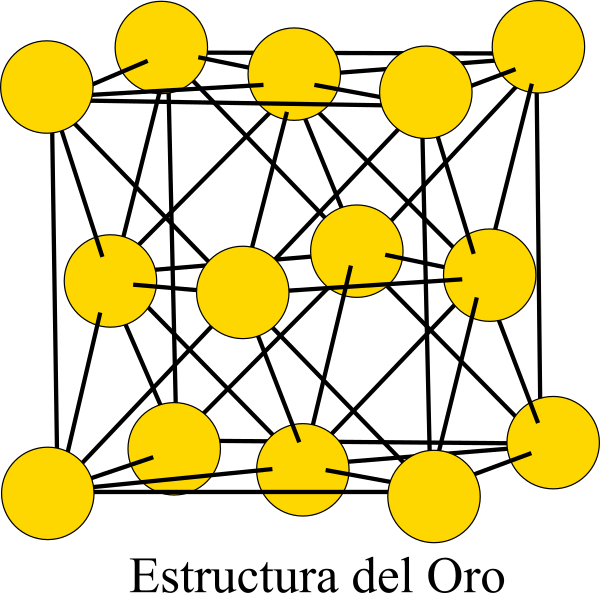
\includegraphics[width=9cm]{Imagenes/estructura-oro}
				\caption[Estructura atómica del oro]{Esquema de la estructura atómica de oro que conforma la cristalización octahedral, modificado de \citet{sorrell1973}}.
				\label{fig:eo}
			\end{figure}
			
			Los métodos Geoeléctricos se clasifican en dos grupos, métodos pasivos y de inducción, los primeros corresponden a aquellos en los que se mide el potencial eléctrico natural, usualmente medido en mili volts, en donde se requiere de electrodos no polarizables para tener medidas lo más claras posibles; mientras que los métodos de inducción emplean un arreglo de electrodos, o inductores de campo electromagnéticos, mediante los cuales se induce un campo eléctrico al subsuelo, calculando la diferencia de potencia eléctrica en el medio, o bien, el decaimiento de la polarización inducida \citep{revil2013, reynolds2011, igboama2023}.
			
			Los métodos de inducción, Sondeo Eléctrico Verticales (VES, por sus siglas en inglés), Tomografía de Resistividad Eléctrica (ERT, por sus siglas en inglés), Polarización Inducida (IP, por sus siglas en inglés), presentan una gran ventaja ya que no dependen del medio para poder realizar una lectura, ademas de poder realizarlos en cualquier momento, manteniendo el equipo en condiciones de operación, y pode diseñar arreglos de adquisición que nos permitan tener un muestreo tan amplio o limitado como sea conveniente, solo limitados por el alcance y potencia de los equipos empleados. Por otro lado su interpretación presenta un alta ambigüedad, solo acotado por la cantidad de referencias que puedan cruzarse para robustecer el modelo geológico y de inversión, y así poder llegar a una interpretación satisfactoria \citep{reynolds2011, igboama2023}.
			
			El método de prospección geoeléctrica, en especifico el SEV y la TRE, consiste en determinar la distribución de resistividades del subsuelo, de manera que se pueda establecer una correlación entre la resistividad y un modelo ajustado a la realidad geológica-estructural, geotécnica o geohidrológica del objeto de estudio.
	
		\subsection{Sondeo Eléctrico Vertical}
			
			Los SEV corresponden al método de mas rápida ejecución y económicamente mas accesible, por lo que es ampliamente empleado para solucionar problemas de ingeniería, minería, geotecnia, monitoreo e impacto ambiental y abastecimiento de Aguas potable; siendo de gran utilidad en la exploración de hidrogelogica ya que la respuesta resistiva de un medio saturado permite establecer diferencias concisas y discriminar entre agua dulce, salada, rocas fracturadas, arcillas , arenas, conglomerados, etc.
			
			La resistividad es medida mediante la inyección de una corriente en el subsuelo y mientras que se monitorea y captura la diferencia de potencial eléctrico en la superficie, esta lectura corresponde al valor de la contribución resistiva de todas las capas por donde fluye la corriente.
			
			La inyección de corriente y medición del potencial se realiza a través de un arreglo de dos pares de electrodos, $A, B (C_{1}, C_{2})$ y $M, N (P_{1}, P_{2}) $ respectivamente, siendo el electrodo $A (C_{1})$ el polo positivo y $B (C_{2})$ el polo negativo de inyección, mientras que el electrodo $M (P_{1})$ corresponde al polo positivo y $N (P_{2})$ al polo negativo de los electrodos de potencial.\\
			 
			\begin{figure}[h!]
				\centering
				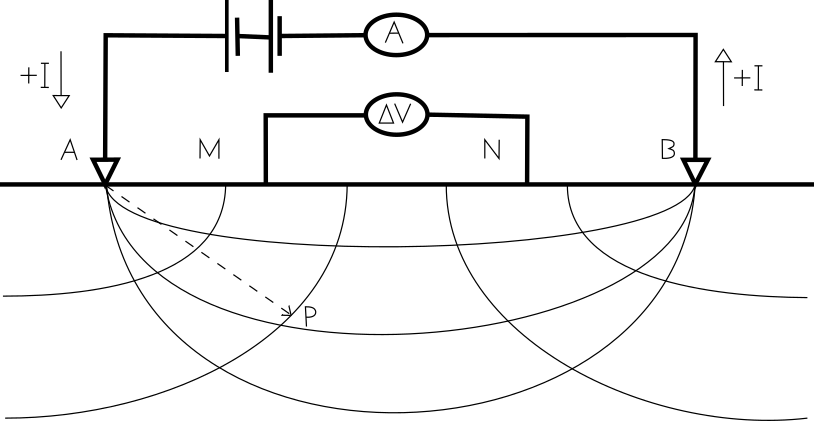
\includegraphics[width=9cm]{Imagenes/ArregloElectrodos}
				\caption[Configuración general de electrodos]{Configuración general de arreglo de electrodos, modificado de \citet{reynolds2011}}.
				\label{fig:AE}
			\end{figure}
			La resistividad del subsuelo se calcula a partir de la ley de Ohm, considerando el caso general en donde el medios es homogéneo y el arreglo de electrodos presenta una distribución convencional, donde se establece una relación directamente proporcional entre la la resistencia $R$ ,medida en Ohm ($\Omega$), y el cociente entre la diferencia de potencial $\Delta V$ y la corriente inducida $I$, para un valor puntual \citep{igboama2023}.
			
			\begin{equation}
				R = \frac{\Delta V}{I}
			\end{equation}
			   
			Sabiendo que se puede calcular $R$ para una sección con longitud $L$ y un área $A$, transversal del material, conociendo la resistividad ($\rho$) del material \citep{igboama2023, lowrie2020}, podemos reescribir la ecuación como: 
			
			\begin{equation}
				R = \rho \frac{L}{A}  \rightarrow  	\rho  = R \frac{A}{L} \rightarrow \rho  = R \cdot k
			\end{equation}
			
			Donde la resistividad ($\rho$) es una constante de proporcionalidad del medio y $k$ es el factor geométrico de distribución del flujo de corriente en términos de la del arreglo  de los electrodos de inducción y potencial (distancias entre los electrodos A-M-N-B ) \citep{igboama2023, lowrie2020}.
			
			\begin{equation}
				k = 2\pi \left(  \dfrac{1}{AM} - \dfrac{1}{AN} - \dfrac{1}{BM} + \dfrac{1}{BN} \right) 
			\end{equation}
			
			Tenemos que la resistividad aparente ($\rho _{A}$) de una sección del subsuelo, corresponde a la contribución resistiva de las unidades geológicas en esa sección, en términos de las distancias entre electrodos, la diferencia de potencial y el flujo de corriente en el medio \citep{igboama2023, lowrie2020}, esta dado por la siguiente ecuación:
			
			\begin{equation}
				\rho_{A} = \frac{\Delta U}{I} \cdot k %\rho_{A} = 2\pi \cdot \frac{\Delta U}{I} \cdot k
			\end{equation}
			
			\subsubsection{Arreglo de Electrodos y Factor Geométrico}
			
				Cada arreglo presenta ventas, desventajas, rango de sensibilidad y espacio de ejecución, debido a estas características y se tiene que evaluar e identificar que arreglo cumple con las condiciones adecuadas para ser ejecutado, considerando el espacio disponible en el sitio de estudio, el nivel de ruido (motores, conexiones a tierra mal aterrizadas, antenas, postes metálicos, arboles), la profundidad de objeto de prospección y la resolución vertical alcanzable (ver figura \ref{fig:Contri}).
				
					\begin{figure}[h!]
						\centering
						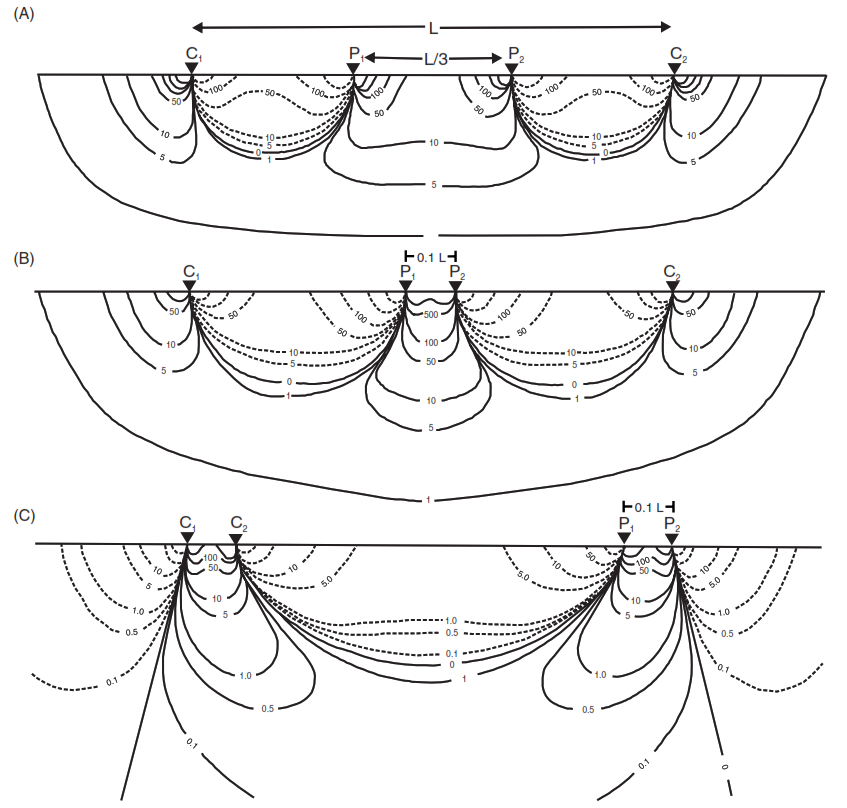
\includegraphics[width=12cm]{Imagenes/5}
						\caption[Esquema de la contribución de la respuesta eléctrica]{Esquema de la contribución de la respuesta de resistividad eléctrica, modificado de \citet{reynolds2011}}.
						\label{fig:Contri}
					\end{figure}				
				
				Como se observa en la sección anterior, la resistividad se determina empleando una configuración de los electrodos durante una medición, las distintas configuraciones de electrodos se encuentran ampliamente documentadas, cada una presenta un factor geométrico distinto \citep{igboama2023, lowrie2020}, los principales arreglos geoeléctricos son:
				
				\begin{description}
					\item[Wenner ]  
							\begin{equation}
								\rho_{A} = 2\pi \cdot R \cdot a
							\end{equation}
							
							\begin{figure}[h!]
								\centering
								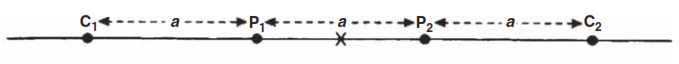
\includegraphics[width=9cm]{Imagenes/1}
								\caption[Esquema del arreglo Wenner]{Esquema del arreglo Wenner, modificado de \citet{reynolds2011}}.
								\label{fig:AW}
							\end{figure}
							
					\item[Schlumberger ] 
					
						\begin{equation}
							\rho_{A} = \frac{\pi a^{2}}{b} \left[ 1 - \frac{b^{2}}{4 a^{2}} \right] \cdot R, \quad a \geq 5b
						\end{equation}

							\begin{figure}[h!]
								\centering
								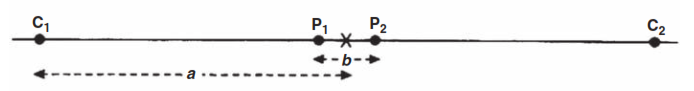
\includegraphics[width=9cm]{Imagenes/2}
								\caption[Esquema del arreglo Schlumberger]{Esquema del arreglo Schlumberger, modificado de \citet{reynolds2011}}.
								\label{fig:AS}
							\end{figure}
					
					\item[Dipolo-dipolo]  
					
							\begin{equation}
								\rho_{A} = \pi n(n+1)(n+2)a \cdot R
							\end{equation}
					
							\begin{figure}[h!]
								\centering
								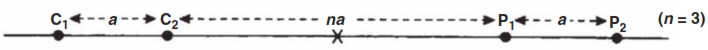
\includegraphics[width=9cm]{Imagenes/3}
								\caption[Esquema del arreglo Dipolo-dipolo]{Esquema del arreglo Dipolo-dipolo, modificado de \citet{reynolds2011}}.
								\label{fig:ADD}
							\end{figure}
				\end{description}
	
	\section{Adquisición de Datos Geofísicos}
	
	Previo al trabajo de adquisición se realiza un análisis de entorno, en el cual se verifica la viabilidad del arreglo dadas las condiciones del sitio, considerando lo siguiente: espacio disponible en el sitio de estudio, profundidad de exploración, nivel de ruido eléctrico, interferencias con la estabilidad del potencial natural del subsuelo, profundidad del objeto de exploración y dimensiones aproximadas del mismo.
	
		\subsection{Intervalo de Muestreo en SEV}
			
			El intervalo de muestreo empleado durante la adquisición de un SEV es un parámetro crítico que influye en la calidad y precisión de los datos geofísicos adquiridos, ya que esta estrechamente relacionado con la resolución vertical que deseamos de acuerdo al objeto de estudio. Durante la planeación es necesario considerar distintas condiciones, como son:
			
			\begin{itemize}
				\item Los espesores de cada unidad.
				\item La distribución de las distintas unidades.
				\item Profundidad de investigación
				\item Ruido en la señal.
			\end{itemize}
			
			Para establecer un intervalo de muestreo apropiado, se deben considerar el Teorema de Muestreo de Nyquist y El teorema de Shannon-Hartley (teorema de codificación de canal ruidoso)
			
			El Teorema de Muestreo de Nyquist, el cual, es un principio fundamental en el procesamiento de señales analógicas y digitales, donde establece las condiciones mínimas necesarias para una reconstrucción una señal analógica a partir de muestras discretas \citep{alvarado2010}.
			
			El teorema de muestreo de Nyquist nos garantiza las condiciones necesarias y suficientes para llevar a cabo una adquisición exitosa de muestreo de una señal, llámese distribución de resistividad en un medio heterogéneo y discontinuo \citep{alvarado2010}.
			
			\begin{equation}
				f_{s} \geq 2 \cdot f_{max}
			\end{equation}
			
			Donde la frecuencia de muestreo $f_{s}$ es por lo menos dos veces mayor a la frecuencia máxima $f_{max}$ conocida, cuando el teorema no se cumple se genera una distorsión en la señal, sumando las frecuencias altas incompletas a la señal natural de baja frecuencia, generando ruido, y problemas de interpretación, se conoce como aliasing \citep{alvarado2010}. 
			
			Considerando el medio geológico como una región con presencia coanstante de ruido electrico de fuentes tanto naturales como humanas, es impresindible considerar el teorema de Shannon-Hartley aplicando apilamiento de muestreo como metodo de reduccion de la relacion ruido señal, durante la adquisicion de datos; esto quiere decir calcular el promedio de muestreos cointinuos en un intervalo definido de aperturas entre electrodos.
			
			%% agregar ecuacion de shanon y desgrlosar sus elementos e interpretacion
				
			\subsubsection{Factores que Determinan el Intervalo de Muestreo}
		
				En el contexto de la adquisición de datos mediante SEV, el intervalo de muestreo es equivalente al espaciado entre puntos donde se realizan mediciones de resistividad del subsuelo. Este intervalo de muestreo debe ser lo mas pequeño posible, de modo que permita obtener muestras de resistividad \citep{telford1990}, esta relación se define de la siguiente manera:
				
				\begin{equation}
					f_{s}= \frac{1}{\Delta x}
				\end{equation}
				
				donde el intervalo de muestreo $\Delta x$ debe ser menor a la mitad de la longitud de onda ($\lambda_{min}$, espesor) asociado al objetivo de exploración
				
				\begin{equation}
					\Delta x \leq \frac{\lambda_{min} }{2}
				\end{equation}
				
				
			
		\subsection{Proceso de Adquisición In Situ}
			La adquisición de datos se realiza mediante la lectura directa en campo, al inducir corriente continua empleando un resistivimetro mediante de los electrodos de corriente A ($C_{1}$) y B ($C_{2}$), mientras se realiza la lectura de potencia en los electrodos M ($P_{1}$) y N ($P_{2}$), la lectura se realiza en intervalos regulares en instantes de inyección de corriente distintos \citep{telford1990}.
			
			Durante la toma de datos es importante considerar los modelos previos realizados durante el análisis preliminar, ya que las resistividades esperadas para las unidades, permiten tener control en la dispersión de datos, identificando tomas erróneas y corrigiendo al momento con una nueva lectura \citep{telford1990}.
	
	\section{Machine Learning (ML) en la Geofísica}  
	
	La aplicación de ML y el DL en la geofísica es ampliamente utilizado en exploración sísmica, abarcando los procesos de adquisición, procesado e interpretación, mejorando los tiempos de procesamiento, clasificación e interpretación, ya que es en este método donde se cuenta con la mayor cantidad de datos para entrenamiento \citep{wrona2018}; en menor medida se implementan técnicas de ML en la exploración y prospección geoeléctrica, hay algunos ejemplos destacables como son \cite{liu2020, el2001, li2024}, sin embargo no es un estándar en la industria, pese a las ventajas que puede tener su aplicación, como es el caso de este estudio
		
	El aprendizaje automático o machine learning, son un conjunto de técnicas que utilizan algoritmos con los cuales permite a un sistema aprender y generar predicciones, para lo que requiere un conjunto de datos para poder realizar el entrenamiento. Podemos clasificar los algoritmos de ML de dos maneras, por el tipo de aprendizaje, correspondiendo a Aprendizaje supervisado, no supervisado y por refuerzo, y por la relación que establecen con los parámetros del conjunto de datos de entrenamiento, es decir, modelos paramétricos y no paramétricos \citep{li2024}. 
	
	De los modelos no paramétricos destacan por su adaptabilidad a la estructura subyacente de los datos, por lo que pueden realizar aprendizaje de relaciones complejas entre datos, así como ausentes de linealidad, teniendo un costo en volumen de datos, requiriendo un número mayor para su entrenamiento, destacan los algoritmos siguientes.
	
	\begin{itemize}
		\item Árboles de decisión
		\item Random Forests
		\item K-Nearest Neighbors (KNN)
		\item Máquinas de soporte vectorial (kernelizados)
	\end{itemize}
	
	Dada la naturaleza de los datos de SEV's, heterogéneos, discontinuos y no lineales, es conveniente abordar su analistas desde un enfoque no paramétrico, teniendo esto en cuanta, la técnica Random Forests destaca siendo eficaz en la tarea de clasificación y regresión, teniendo algunos beneficios como son la reducción del sobre ajuste, interpretación de variables, resistencia al aliasing.
	
	\section{Random Forests} 
	
		La técnica Random Forests emplea múltiples arboles de decisión independientes entre si, donde cada árbol realiza una votación de clases, donde se selecciona la más popular de la entrada de cada árbol realizando una combinación de salida, permitiendo realizar una clasificación de características complejas o realizar regresiones de datos complejos multivariables \citep{breiman2001, lan2020}.
		
		La herramienta de Random Forests, de acuerdo con \citet{breiman2001} emplea tres elementos clave en el proceso de entrenamiento, bagging, selección aleatoria de características y agregación por votación, resultando en la combinación del los resultados en una predicción o clasificación robusta y ajustada \citep{lan2020}.
		
		\subsection{Siembra del bosque}
		
			\citet{breiman2001} nos dice que Random Forests es un conjunto de clasificadores $H(x,\theta_{k})$, $x$ es un vector de entrada y $\theta_{k}$ corresponden a vectores aleatorios independientes.
			
			A partir de los datos de entrada, se generan subconjuntos de datos de entrenamiento, estos se seleccionan con cierta aleatoriedad empleando la técnica bootstrap sampling, en cada nodo de los subconjuntos de entrenamiento se selecciona un subconjunto de características por votación de popularidad, dejando crecer cada árbol sin realizar poda hasta completar los criterios de finalización, es decir un numero de instancias preestablecido\citep{breiman2001}.
			
		\subsection{Predicciones del bosque}
		
			
			 La salida de un Random Forest para una entrada $x$ se basa en las predicciones individuales de los árboles para cada clase $h_{k}(x)$, se realiza un conteo de cada clase, producto de la predicción de cada árbol, sumando las salidas $I(h_{k}(x)=c)$, y finalmente se selecciona clase con mayor numero de predicciones, obteniendo la predicción de clasificación $H(x)$,donde $x$ es una función indicadora que vale 1 si $h_{k}(x)=c$, y $0$ en caso contrario \citep{breiman2001}.
			
			\begin{equation}
				H(x) = \text{argmax}_c \sum_{k=1}^K I(h_k(x) = c)
			\end{equation}

			
			El proceso de la regresión se obtiene a partir de la media aritmética de cada predicción individual, donde cada árbol produce un valor numérico $h_{k}(x)$ correspondiente a cada $x$, al corresponder con promedio de las predicciones se le otorga mas estabilidad cuando tenemos un numero elevado de arboles  y un conjunto de datos grande, entendiéndolo como un modelo central que incorpora información de cada árbol \citep{breiman2001}. 
			
			\begin{equation}
					H(x) = \frac{1}{K} \sum_{k=1}^K h_k(x)	
			\end{equation}

		\subsection{Margen y Error de Generalización}
		\subsection{Robustez y Convergencia}
		\subsection{Aplicaciones de Random Forests en Geofísica}
	
\chapter{METODOLOGÍA}

\section{ideas y apuntes}

faltan las referencias....

Esta investigación propone la implementación de un modelo de Random Forests (Bosques Aleatorios) para mejorar la calidad y optimización del proceso de adquisición de datos durante un Sondeo Eléctrico Vertical (SEV). El objetivo es utilizar técnicas de aprendizaje automático para clasificar las lecturas obtenidas y generar una regresión que permita sugerir intervalos de muestreo adicionales, mejorando así la exploración geofísica.

El flujo de trabajo propuesto consta de las siguientes etapas:

Adquisición de datos y preprocesamiento: En primer lugar, se realiza la adquisición de datos in situ utilizando el método de Sondeo Eléctrico Vertical (SEV), el cual consiste en medir la resistividad del terreno a diferentes profundidades con un intervalo de muestreo predefinido. Este intervalo se determina de acuerdo con el objetivo de exploración, como la identificación de unidades geológicas, acuíferos, fallas, fracturas o estructuras antropogénicas. Para garantizar que los datos sean adecuados para el análisis, se lleva a cabo un preprocesamiento de los datos, que incluye la limpieza de valores atípicos, normalización de las lecturas y manejo de valores faltantes.

Clasificación de las lecturas con Random Forests: Se emplea el algoritmo Random Forests, una técnica de aprendizaje automático no paramétrica que consiste en crear múltiples árboles de decisión que luego se combinan para mejorar la precisión del modelo. El modelo se entrena utilizando las lecturas de resistividad obtenidas de las distintas profundidades y las características asociadas (como el tipo de terreno, las propiedades geológicas conocidas o las variables del sondeo). Los árboles se entrenan para clasificar los datos en diferentes categorías, tales como las unidades geológicas presentes, los acuíferos, las fracturas, entre otros. La clasificación permitirá identificar patrones en las lecturas de resistividad que corresponden a diferentes tipos de formaciones geológicas.

Generación de la regresión para optimizar el intervalo de muestreo: Una vez que se haya realizado la clasificación, se utiliza el modelo de regresión basado en Random Forests para predecir la resistividad eléctrica en profundidades no muestreadas. Esto permitirá estimar la resistividad del terreno en puntos específicos que no han sido cubiertos por el muestreo inicial. A partir de estas predicciones, se podrán proponer intervalos de muestreo adicionales in situ que mejoren la representación de las formaciones geológicas de interés. La regresión también proporcionará un modelo predictivo que puede ajustarse dinámicamente para adaptar los intervalos de muestreo según las características del terreno y los objetivos de exploración.

Evaluación del modelo y ajuste de parámetros: Se realiza una evaluación exhaustiva del modelo mediante técnicas de validación cruzada para asegurarse de que el modelo esté bien entrenado y sea capaz de generalizar correctamente a nuevos datos. Además, se compara el rendimiento del modelo de Random Forests con otras técnicas de clasificación y regresión para determinar su eficacia en comparación con otros enfoques. Se analizan métricas como la precisión en la clasificación, el error cuadrático medio (RMSE) en la regresión y la capacidad de predicción en términos de muestreos adicionales.

Optimización y mejora continua: Finalmente, se optimizan los parámetros del modelo (como el número de árboles y la profundidad de los mismos) para mejorar la precisión y eficiencia del modelo. A medida que se incorporan nuevos datos de exploración y se obtienen más lecturas de resistividad, el modelo puede ser recalibrado y ajustado para mantener su efectividad en la identificación de objetivos geofísicos y en la optimización del intervalo de muestreo.


En la implementación de técnicas avanzadas como Machine Learning (ML), modelos como Random Forests pueden analizar patrones en los datos y predecir áreas con alta variabilidad de resistividad. Esto permite:

Ajustar dinámicamente el intervalo de muestreo durante la adquisición \textit{in situ}.
Generar muestreos adicionales en áreas críticas para aumentar la precisión.
Con este enfoque, se asegura que el intervalo de muestreo esté alineado con el teorema de Nyquist, optimizando la calidad de los datos y reduciendo la redundancia.

El uso de Random Forests permite abordar la complejidad y la variabilidad inherentes al proceso de adquisición de datos en el contexto de exploración geofísica. Este enfoque optimiza el proceso de muestreo, mejora la calidad de los datos obtenidos y proporciona una base para generar predicciones más precisas, contribuyendo así al éxito de las campañas de exploración.

\section{Variables de Entrada}
	Al observar las ecuaciones 5.1, 5.3 y 5.4, es posible identificar las variables involucradas en el calculo de la resistividad aparente, estos valores son medidos por un equipo automático o bien, de forma manual a través de la lectura directa en un resistivímetro, para lo cual se requiere de comprobaciones durante la adquisición.
		
	Como observamos en la tabla \ref{tab:T1}, se integran datos generados durante la planeación y valores medidos en la etapa de adquisición; Z= profundidad aparente de exploración; K= factor geométrico; AB/2= apertura total de muestreo entre dos;  MN= distancia entre electrodos de potencial; Pn= potencial natural; Pi= potencial inducido; I= corriente Inducida; PPn= promedio del potencial natural; PPi= promedio de potencial inducido; U= diferencia entre PPn y PPi; PI= promedio de corriente inducida; Rha= resistividad aparente ponderada.
	
	
	
% Please add the following required packages to your document preamble:
% \usepackage{graphicx}
% \usepackage[table,xcdraw]{xcolor}
% Beamer presentation requires \usepackage{colortbl} instead of \usepackage[table,xcdraw]{xcolor}
\begin{table}[]
	\resizebox{\columnwidth}{!}{%
		\begin{tabular}{c|c|c|c|c|c|l|l|l|l|l|l|l|l|l|l|l|l|l|l}
			\rowcolor[HTML]{C0C0C0} 
			\textbf{Z} & \textbf{K} & \textbf{AB/2} & \textit{\textbf{AB/5  \textgreater{}}} & \textit{\textbf{MN}} & \textit{\textbf{\textgreater AB/20}} & \multicolumn{1}{c|}{\cellcolor[HTML]{C0C0C0}\textbf{Pn}} & \multicolumn{1}{c|}{\cellcolor[HTML]{C0C0C0}\textbf{Pi}} & \multicolumn{1}{c|}{\cellcolor[HTML]{C0C0C0}\textbf{I}} & \multicolumn{1}{c|}{\cellcolor[HTML]{C0C0C0}\textbf{Pn}} & \multicolumn{1}{c|}{\cellcolor[HTML]{C0C0C0}\textbf{Pi}} & \multicolumn{1}{c|}{\cellcolor[HTML]{C0C0C0}\textbf{I}} & \multicolumn{1}{c|}{\cellcolor[HTML]{C0C0C0}\textbf{Pn}} & \multicolumn{1}{c|}{\cellcolor[HTML]{C0C0C0}\textbf{Pi}} & \multicolumn{1}{c|}{\cellcolor[HTML]{C0C0C0}\textbf{I}} & \multicolumn{1}{c|}{\cellcolor[HTML]{C0C0C0}\textbf{PPn}} & \multicolumn{1}{c|}{\cellcolor[HTML]{C0C0C0}\textbf{PPi}} & \multicolumn{1}{c|}{\cellcolor[HTML]{C0C0C0}\textbf{U}} & \multicolumn{1}{c|}{\cellcolor[HTML]{C0C0C0}\textbf{PI}} & \multicolumn{1}{c}{\cellcolor[HTML]{C0C0C0}\textbf{Rha}} \\ \hline
			\rowcolor[HTML]{FFFFFF} 
			\textbf{1.8} & \textbf{56.549} & \textbf{3} & \textit{\textbf{1.2}} & \textit{\textbf{0.5}} & \textit{\textbf{0.3}} & 1 & 6 & 15 & 0 & 6 & 15 & 0 & 5 & 15 & 0.3 & 5.7 & 5.3 & 15.0 & 20.11 \\ \hline
			\rowcolor[HTML]{FFFFFF} 
			\textbf{2.4} & \textbf{100.531} & \textbf{4} & \textit{\textbf{1.6}} & \textit{\textbf{0.5}} & \textit{\textbf{0.4}} & 12 & 19 & 3 & 0 & 25 & 17 & 5 & 24 & 13 & 5.7 & 22.7 & 17.0 & 11.0 & 176.45 \\ \hline
			\rowcolor[HTML]{FFFFFF} 
			\textbf{3} & \textbf{157.080} & \textbf{5} & \textit{\textbf{2}} & \textit{\textbf{0.5}} & \textit{\textbf{0.5}} & 8 & 54 & 73 & 8 & 52 & 85 & 8 & 40 & 83 & 8.0 & 48.7 & 40.7 & 80.3 & 80.28 \\ \hline
			\rowcolor[HTML]{FFFFFF} 
			\textbf{3} & \textbf{31.416} & \textbf{5} & \textit{\textbf{2}} & \textit{\textbf{2.5}} & \textit{\textbf{0.5}} & 52 & 508 & 42 & 52 & 648 & 72 & 52 & 606 & 21 & 52.0 & 587.3 & 535.3 & 45.0 & 476.64 \\ \hline
			\rowcolor[HTML]{FFFFFF} 
			\textbf{4.8} & \textbf{80.425} & \textbf{8} & \textit{\textbf{3.2}} & \textit{\textbf{2.5}} & \textit{\textbf{0.8}} & 48 & 60 & 6 & 48 & 62 & 7 & 51 & 59 & 4 & 49.0 & 60.3 & 11.3 & 5.7 & 160.85 \\ \hline
			\rowcolor[HTML]{FFFFFF} 
			\textbf{6} & \textbf{125.664} & \textbf{10} & \textit{\textbf{4}} & \textit{\textbf{2.5}} & \textit{\textbf{1}} & 52 & 60 & 2 & 52 & 60 & 5 & 52 & 60 & 5 & 52.0 & 60.0 & 8.0 & 4.0 & 301.59 \\ \hline
			\rowcolor[HTML]{FFFFFF} 
			\textbf{9} & \textbf{282.743} & \textbf{15} & \textit{\textbf{6}} & \textit{\textbf{2.5}} & \textit{\textbf{1.5}} & 52 & 76 & 54 & 52 & 78 & 87 & 50 & 64 & 44 & 51.3 & 72.7 & 21.3 & 61.7 & 100.04
		\end{tabular}%
	}
	\caption{Ejemplo de atributos empleados en el calculo de la resistividad aparente.}
	\label{tab:T1}
\end{table}
	
	En términos generales, el proceso de adquisición consiste en la inducción de una corriente eléctrica a través del medio geológico, dicha intensidad de corriente es registrada, junto con el valor del potencial natural (Self-Potential) y el potencial inducido, generado por la inyección de corriente a tierra, obteniendo así los elementos necesarios para calcular el valor de la resistividad, habiendo previamente planeado la configuración geométrica del arreglo.

	\subsection{Datos de entrada}
		
		Para los datos de entrada se emplearon levantamientos de SEV previamente procesados e interpretados en correlación con muestreo directo por sondeo de penetración estándar (SPT por sus siglas en inglés), correspondientes a ambiente de deposito sedimentario y flujos volcánico, en ambos caso subyaciendo a unidades sedimentarias recientes.
		
		A partir de estos resultados etiquetados, valores de resistividad aparente, es como de modela variaciones, modificando el espesor de las unidades, ya que cada muestreo de resistividad aparente integra la respuesta conjunta de las unidades que la preceden, es decir las capas geoeléctricas por arriba de la profundidad aparente de exploración, para iguar las condiciones en los modelos que integran los datos de entrenamiento, se emplea la Librería PyGIMLI, la cual esta preparada para realizar esta tarea.
		
		\subsubsection{Limpieza de datos}
		
		\subsubsection{Generación de valores SEV’s}
		
		\subsubsection{Resistividad aparente}
		
		\subsubsection{Atributos cualitativos asociados a la curva de resistividad}


	\subsection{Clasificación, transformación y escalado de los datos}
		\subsubsection{Normalización o estandarización de resistividades si se observan grandes variaciones}
		\subsubsection{Transformación logarítmica de resistividad para reducir el sesgo de valores extremos}
		\subsubsection{Codificación de categorías litológicas si se incluyen como variable adicional}

\section{Diseño del Modelo Random Forest}
	\subsection{Regresión}
	\subsection{Configuración inicial del modelo, numero de árboles, profundidad, muestras y muestra mínima}
	\subsection{Configuración y optimización de hiperparametros}

\section{Preparación del dataset para la implementación del modelo}

\section{Implementación del modelo}
\subsection{Entrenamiento del modelo}
\subsection{Mapas de probabilidad y entrenamiento de regresión}

\section{Evaluación del modelo}
	\subsection{Regresión y validación cruzada}
	\subsection{Análisis de incertidumbre}


\section{Reporte estadístico}
\chapter{RESULTADOS Y CONCLUSIONES}

\appendix
%%% Haz un documento para cada apéndice, si es que tienes
\chapter{Apéndice I}






\backmatter
\pagestyle{main}

% Aquí va la bibliografía, puedes usar el entorno de LaTeX (thebibliography)
% o la herramienta BibTeX. En caso de que optes por BibTeX, puedes usar
% alguno de los archivos de estilo (mighelbib.bst o mighelnat.bst) incluidos
% en el paquete, cuyos diseños armonizan con el diseño de tesis provisto por
% fime.cls. Para muestra, basta un botón:
\bibliographystyle{mighelnat}
\bibliography{MiBiblio}

\label{lastpage}
%%Autobiografia

\chapter*{Resumen autobiográfico}
\thispagestyle{empty}

\begin{center}
\autor

Candidato para obtener el grado de\\
\grado\\
\orientacion\bigskip

\uanl\\
\fcfm\bigskip

Tesis:\\
\textsc{\large\titulo}
\end{center}\bigskip

%Aquí va tu historia
Aquí va tu historia. Recuerda que debe incluir: lugar y fecha de nacimiento, nombre de los padres, escuelas y universidades en las que se graduó después de la preparatoria, títulos o grados obtenidos (no incluir los estudios que se están concluyendo), experiencia profesional y organizaciones profesionales a las que pertenece (no incluir lista de publicaciones).


\end{document}

